\documentclass[fleqn,10pt]{wlscirep}
\usepackage[utf8]{inputenc}
\usepackage[T1]{fontenc}
\usepackage{graphicx}
\usepackage{amsmath}
\usepackage{csquotes}
\usepackage{pdfpages}
\usepackage{docmute}
\usepackage{filecontents}
\usepackage{listings}
\usepackage{standalone}
\usepackage{subcaption}
\usepackage[
backend=bibtex,
bibstyle=apa,
style=nature,
citestyle=numeric-comp,
]{biblatex}

\addbibresource{bibliography}

\title{YOUR TITLE GOES HERE}

\author[1,*]{AUTHOR1}
\author[1,*]{AUTHOR2}

\affil[*]{EMAIL}

\keywords{KEYWORDS}

\begin{abstract}
... ABSTRACT GOES HERE...
\end{abstract}
\begin{document}

\maketitle

\section*{Introduction}
\subsection{SUBSECTION HEADER GOES HERE}

\section*{Results}
\input{results/Results.tex}

\section*{Discussion}
\subsection{SUBSECTION HEADER GOES HERE}

\section*{Methods}
\subsection{SUBSECTION HEADER GOES HERE}

\begin{figure}
\centering
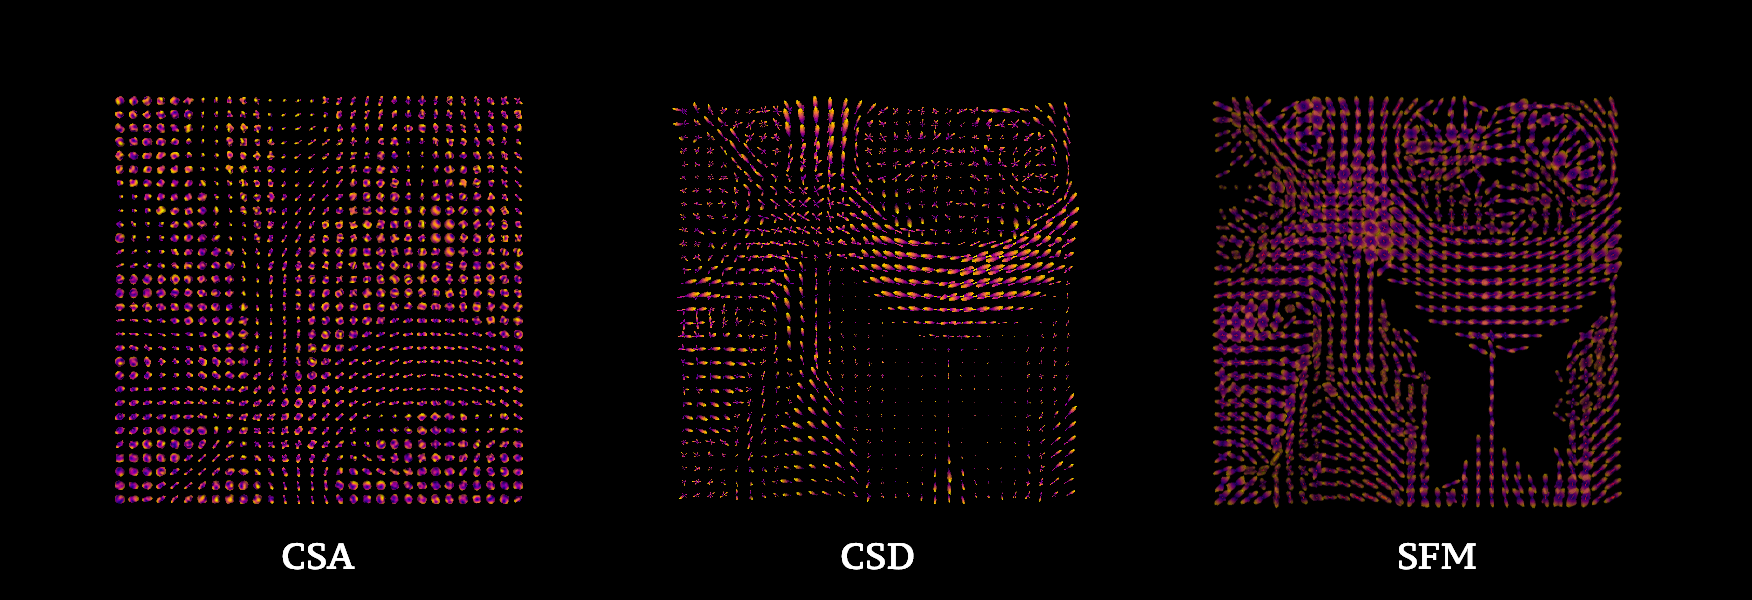
\includegraphics[width=\linewidth, angle=0, scale=1.0, keepaspectratio=true]{figures/SAMPLE_FIGURE_1.png}
\caption{FIGURE1 CAPTION}
\label{fig:FIGURE1_LABEL}
\end{figure}

\begin{figure}
\centering
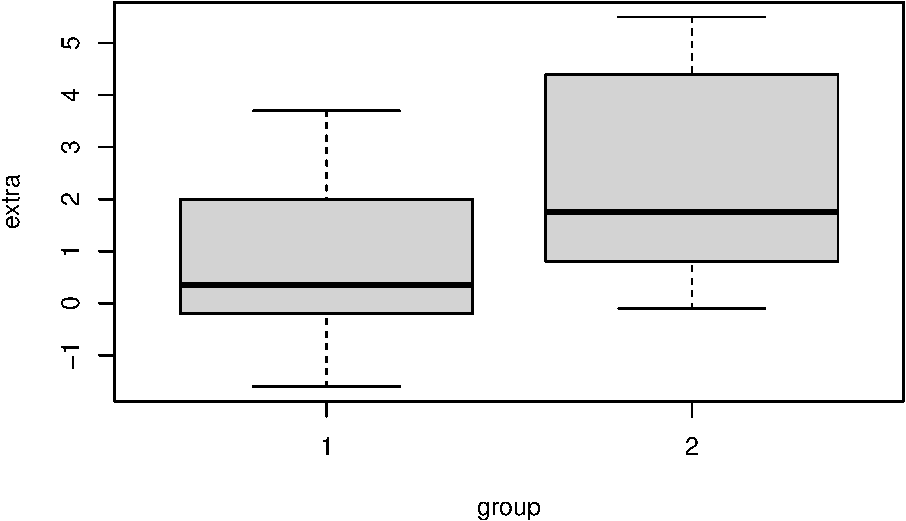
\includegraphics[width=\linewidth, angle=0, scale=1.0, keepaspectratio=true]{figures/T-test-1.pdf}
\caption{FIGURE2 CAPTION}
\label{fig:FIGURE2_LABEL}
\end{figure}

%\begin{table}[ht]
%    \centering
%    \input{results/TABLE1.tex}
%    \caption{TABLE1 CAPTION}
%    \label{tab:TABLE1_LABEL}
%\end{table}

\end{document}